% !TeX spellcheck = en_US
\subsection{Assessing the Performance of the PaSC}
\label{556:Assessment_Eval}
\subsubsection{Setup of the Evaluation}
\label{sec:557_eval_setup}
In comparison to the assessment of the precision and runtime of the quality assessment algorithms, this evaluation is conducted in real-world, distributed deployment with multiple devices. 
The potential for scalability of a centralized, concurrent processing of quality assessment algorithms in comparison to a distributed execution on mobile devices and central servers is assessed.
An application is designed, which consecutively requests quality assessments from the \ac{PaSC} with timing deadlines.
The goal is to increase the rate of completed quality assessments that delivered their results on time.
\paragraph{Algorithms}
To assess the performance of the \ac{PaSC}, we not only use the discussed \ac{RQ}, but also available algorithms for \ac{AQ} and \ac{VQ}.
Each category of algorithms is evaluated independent of the others, offering all resources of our setup solely to the respective assessment category.

The recording quality assessment algorithms address the degradations of camera shake, camera misalignment, and harmful occlusions.
Different algorithms were proposed to analyze and measure the effects of compression in digital video.
Open-source implementations of \ac{NR} algorithms such as BRISQUE~\cite{Mittal2011} (BR), V-BLIINDS (VB)~\cite{Saad2014}, Shrestha et al. (SHR)~\cite{Shrestha2010}, Campanella et al. (CA)~\cite{Campanella2007}, and Saini et al. (SAI)~\cite{Saini2012} are used. 

The analysis of the audio track of \ac{UGV} is discussed.
Besides video quality assessment, algorithms were designed for quality assessment of the audio tracks \cite{ITU-P863}, speech quality analysis \cite{ITU-P563}, 
or specifically, audio degradations in \ac{UGV}~\cite{Li2013}.
\paragraph{Device setup}
The setup of our evaluation consists of a server (Ubuntu 14.04) as well as 15 mobile devices consisting of one Samsung Galaxy S6 (Android 5.1.1), one Sony Xperia Z3 (Android 5.1.1), eight Nexus 5 (Android 6.0) and five Nexus 4 devices (Android 5.1.1).
The devices are categorized into high-end servers and low-end, medium and high-end smartphones.
The classification was validated by the results of the Vellamo\footnote{Qualcomm Vellamo Metal Benchmark; Visited on: 10/09/2016} 
and AnTuTu benchmarks\footnote{AnTuTu Benchmark; \url{http://www.antutu.com/en/index.shtml}, Visited on: 10/09/2016} 
(see Table~\ref{table:556_benchmark}).
\begin{table}[h]
\centering
	\caption[Device setup for the evaluation of the PaSC]{PaSC Evaluation: Performance benchmark results for Vellamo and AnTuTu and categorization of the devices.}
	\begin{tabular}{l c c c c}%{\textwidth}
		& Vellamo & AnTuTu & Class & No\\ \toprule
		\texttt{LG Nexus 4 (N4)} & 600  & 16749 &  low-end & 5\\
		\texttt{LG Nexus 5 (N5)} & 1166 & 26340 & medium & 8\\
		\texttt{Sony Xperia (Z3)} & 1551 & 43911 & high-end & 1\\ 
		\texttt{Samsung Galaxy S6 edge (S6)} & 1569 & 68830 & high-end & 1\\ 
		\bottomrule
		Server & \multicolumn{2}{c}{\specialcell{Intel Xeon (6 cores)\\ 64 GB memory }} & server & 1\\
		\bottomrule
	\end{tabular}
	\label{table:556_benchmark}
\end{table}
\paragraph{Network Setup}
The evaluation setup ensures that the server hosting the algorithm repository is located in the same geographic region - but remote from the mobile devices. 
All runtime statistics are collected on the server, too.

Traffic shaping is used to set the maximum data rate to 50 \unit{$\frac{MBit}{s}$} and a randomly selected minimum latency between 100-300 milliseconds per transmission~\cite{Lampe2013}. 
Higher latencies, e.g., as invoked by the access or backbone network, are included in our results.   
To achieve reliable results, the evaluations were re-performed ten times each. Furthermore, evaluations were scripted with the same configuration parameters, under similar conditions using the same videos.

\paragraph{Scenario}
The evaluation describes an experimental setup in which quality calculation requests are sent continuously by the devices to trigger the selection of an optimal combination of algorithm and device.
At any time 15 assessment requests are processed - thus one request per device. Once completed, another request is created.
The deadlines and accuracy requirements are normalized in the range $[0, 1]$. 
$0$ represents the lowest and $1$ the highest processing time.
The statistics are offered by the algorithm repository of the \ac{PaSC}. 
\ac{PaSC} is compared in both evaluations with an assessment of all algorithms on a central server.

Furthermore, assessments of different quality assessment categories ($AT$) can be run in parallel. 
For each of the evaluated cases metrics are determined - including the average runtime of the quality assessment, the number of successful runs in a given time, and the average utilization.
For the assessment of the runtime, the total time from the request for a quality assessment until the delivery of the result (including transmission and algorithm execution times) is given.
Successful runs are defined as algorithm calculations processed in time for a given deadline. 
The number of successful runs and its relation to the completed runs are metrics indicating if system load and application requirements allow a timely completion of the assessment.
The utilization metric indicates how many resources of the individual devices are used in average.
% -  -  -  -  -  -  -  -  -  -  -  -  -  -  -  -  -  - -
\subsubsection{Utilization of the Devices}
The results of this evaluation are depicted in Figure~\ref{fig:557_PaSC_Results}.
In a first step, the increased utilization by an intelligent selection and placement of the algorithms is shown.
For comparison, a central server instance as described in the system setup section is used. 
As quality assessment requests are made by the application, the average utilization of this single server setup is close to 100\% (97.1\%). 
The rationale behind this is quite obvious: As the number of devices requesting quality assessments is higher than the number of available processors, the resources of the single server are exhausted.
\begin{figure}[!htb]
	\centering
	\subfloat[][]{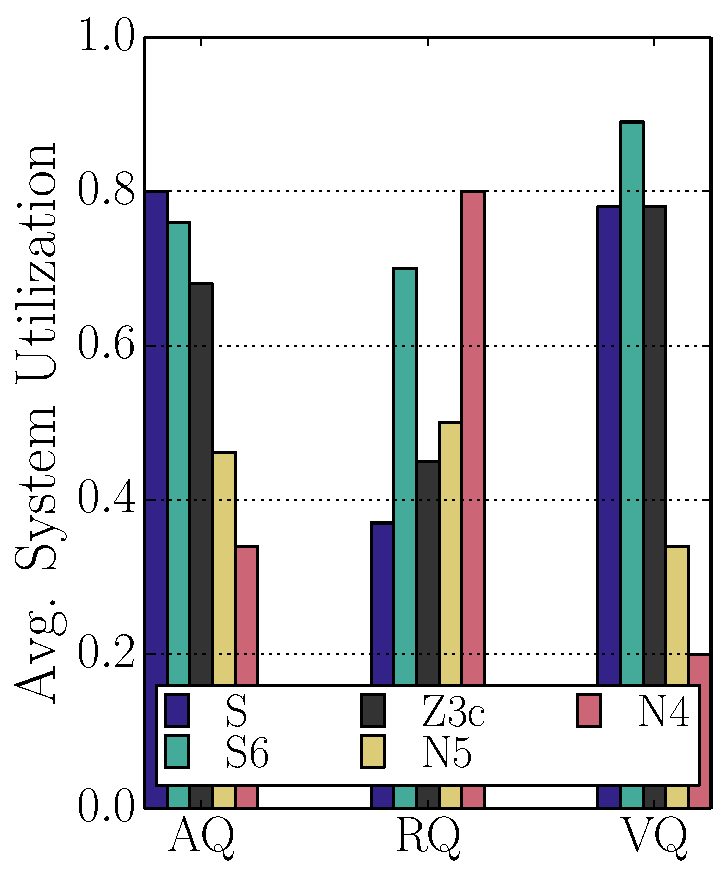
\includegraphics[width=0.245\linewidth]{./gfx/550_QA/diss_Utilization_View1}}
	\subfloat[][]{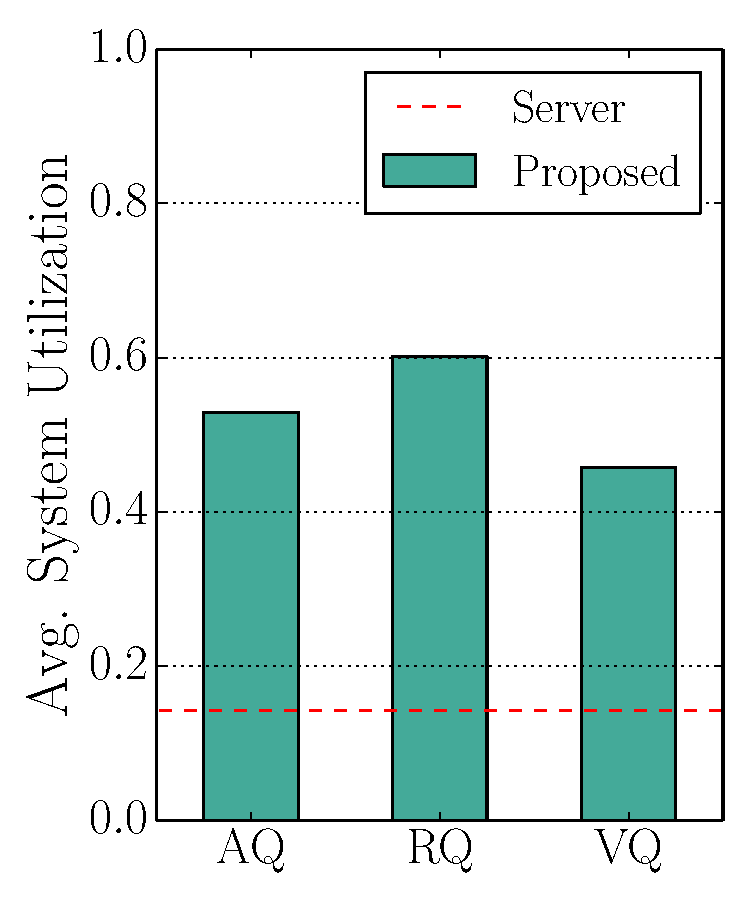
\includegraphics[width=0.245\linewidth]{./gfx/550_QA/diss_Utilization_View2}}
	\subfloat[][]{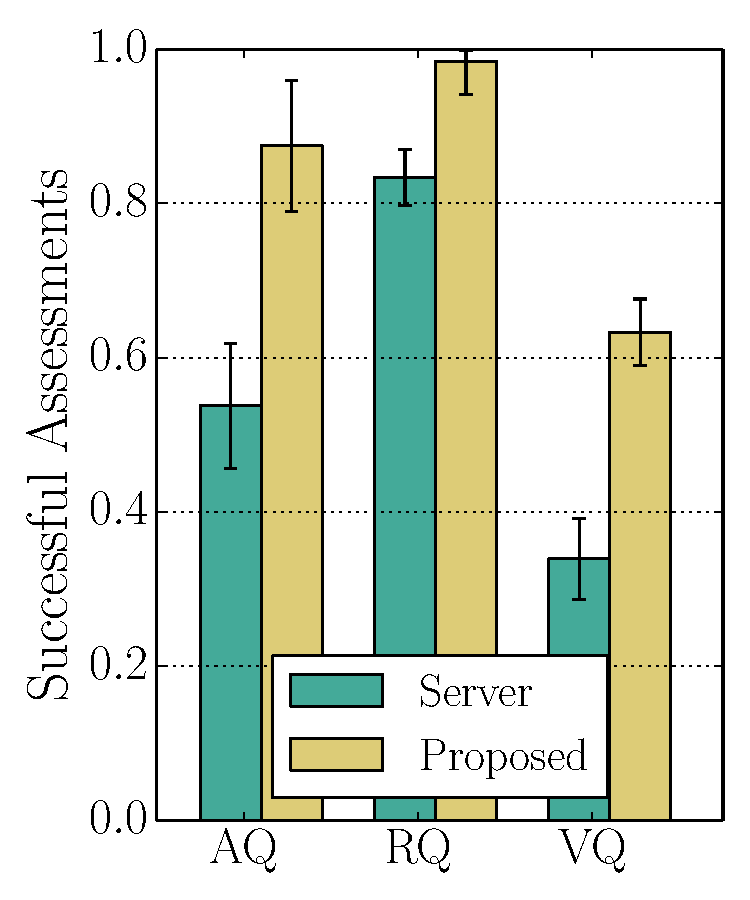
\includegraphics[width=0.245\linewidth]{./gfx/550_QA/diss_SuccesfulRuns}}
	\subfloat[][]{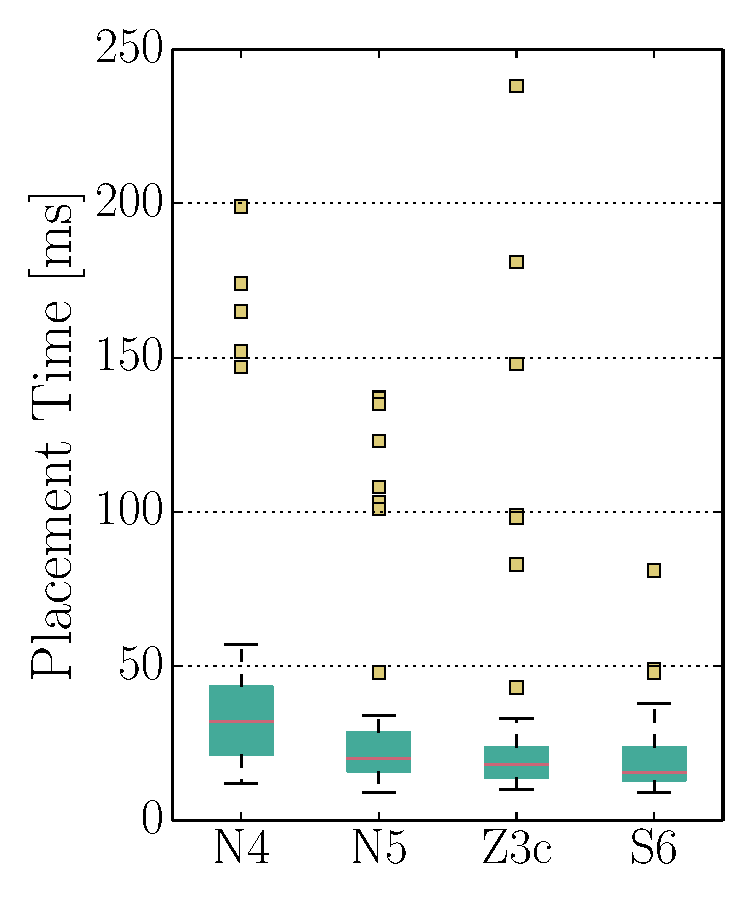
\includegraphics[width=0.245\linewidth]{./gfx/550_QA/diss_runTime}}
	\caption[Evaluation results for using the PaSC]{(a) Average utilization of the different devices when using the PaSC - S: Samsung Galaxy S6 edge, N4: LG Nexus 4, N5: LG Nexus 5, Z3: Sony Experia Z3, S: Server; (b) System utilization averaged and normalized across all devices in the evaluation setup in comparison with a single server; (c) Number of successful quality assessments when hard-timed deadlines are given; (d) Calculation overhead in [ms] for making and distributing a decision in PaSC of which algorithm to run on which device.}
	\label{fig:557_PaSC_Results}
\end{figure}
For the calculation of total system resources, the \ac{CPU} utilization of all devices is sampled with \ac{NTP} synchronized clocks. 
The different processor features (architecture, clock rate, the number of cores) were normalized to retrieve a total utilization score.

In comparison to the single server calculation, Figure~\ref{fig:557_PaSC_Results} illustrates that the \ac{PaSC} distributes different quality assessment tasks to the mobile devices and thus causes a high utilization of resources.
Figure~\ref{fig:557_PaSC_Results} (a) illustrates the average utilization per device and assessment category when using \ac{PaSC}.
The most obvious observation that can be drawn from this figure is that quality assessment tasks are assigned to the devices independent of specific device capabilities. None of the devices reaches its utilization limit (1.0). Especially, weaker devices such as the N4 have only a limited amount of quality assessment tasks in the categories \ac{VQ} and \ac{AQ}, as all algorithms rely on resource-intensive video- or audio-based algorithms.
The \ac{PaSC} is given timing deadlines, which a device must comply with. 
Thus, weaker devices are rather not selected if the algorithm would require a significant processing time.

As the proposed algorithms for \ac{RQ} are using auxiliary sensor input and the related algorithms are computationally less expensive, the quota of assessments on N4 is significantly higher.
At the same time, average utilization of the remaining devices drops.
For \ac{RQ}, it is obvious that offloading works well as the average utilization of the server drops below 0.4.
One of the reasons for the utilization for \ac{RQ} algorithms is that many requests can be executed locally without distribution to remote devices.

Figure~\ref{fig:557_PaSC_Results} (b) depicts, as a result, an average system utilization normalized for all devices.
It depicts the utilization of a single server as a red, dotted line in comparison to the average utilization when using the \ac{PaSC}.
As the number of highly accurate yet lightweight algorithms increases, total system utilization increases significantly. 
The total utilization increases to around 60\% for \ac{RQ} in comparison to a single server installation where only 14.4\% of the system resources are leveraged.
Even for the \ac{VQ} algorithms, the total system utilization increases to above 40\% - thus, more than doubled.
In all cases, utilization increases significantly and the high number of N5 and N4 devices boosts the average utilization for \ac{RQ} in comparison to \ac{AQ} and \ac{VQ}.
Still, one can conclude for the utilization that for all assessment categories, \ac{PaSC} finds sufficient assessment requests to be run on the mobile devices, which significantly reduces the load on the server and enhances scalability.
\subsubsection{Increased Completion of Quality Assessments}
A measure for the effectiveness of the \ac{PaSC} is the number of completed quality assessments.
\ac{PaSC} is perceived as beneficial, if the number of completed quality assessments is significantly higher compared to the centralized processing. 
Figure~\ref{fig:557_PaSC_Results} (c) illustrates a comparison of the single server and the proposed solution regarding successful quality assessments.
Following the description in Section~\ref{sec:557_eval_setup}, a successful quality assessment represents a complete execution of an algorithm and the reporting of the quality result to the requesting application. 

An obvious result is that the ratio of successful (in-time, processed) assessments increase significantly. 
In particular, the complex quality assessment categories \ac{VQ} and \ac{AQ} benefit from the distributed calculation, increasing their rate of successful assessment by 0.2937 and 0.3371. 
Even though they can place only a small number of runs on the weak devices (especially the N4), the more powerful devices such as the S6 and Z3c help to increase the total number of completed assignments. 
For the computationally inexpensive algorithms of the \ac{RQ} category, the ratio increased by 0.1498.

This offloading allows to process more quality algorithms in time.
Note that to allow a fair comparison for evaluating the single server and \ac{PaSC} the total number of assessments is kept constant between the two scenarios.
The \ac{PaSC} would have achieved a significantly higher number of completed assessments in a given time. 
\subsubsection{Influence of Device Heterogeneity}
Besides the effectiveness of the \ac{PaSC}, its efficiency shall be evaluated by inspecting the costs of running the \ac{PaSC} in terms of processing delay and caused network traffic.
Figure~\ref{fig:557_PaSC_Results} (d) shows system processing times, which consist of processing statistics to select an algorithm and the time needed to decide on the algorithm placement.
The time of informing a device to start the processing is also included.

Interestingly, the deployment to different devices affects this decision.
Especially, the low-end devices (N4) need considerably longer time (with a mean of 40 milliseconds) than the high-end devices (S6, Z3c).
Yet, all devices show a significant proportion of outliers which result in selection times of up to 250 milliseconds. 
Such high processing times significantly affect the quality assessments if they are needed for real-time assessments. 
In most cases, the selection and placement processing times take less than 50 milliseconds, which is negligible in comparison to the processing times of the algorithms.
For example, the delay invoked by transmitting sufficient video for algorithm execution lies around 137.5 milliseconds ($\sigma^2 =  27.2$) per video.
The coordination data overhead necessary for using the \ac{PaSC} is rather small at around 20.18 \unit{kB} to 20.41 \unit{kB} per request.
If we consider an average bit rate of 1500\unit{$\frac{KBit}{s}$} for a video stream, the coordination overhead is considerably lower than the video data. 